\documentclass[11pt]{article}

    \usepackage[breakable]{tcolorbox}
    \usepackage{parskip} % Stop auto-indenting (to mimic markdown behaviour)
    \usepackage{sidecap}
    \usepackage{iftex}
    \ifPDFTeX
    	\usepackage[T1]{fontenc}
    	\usepackage{mathpazo}
    \else
    	\usepackage{fontspec}
    \fi

    % Basic figure setup, for now with no caption control since it's done
    % automatically by Pandoc (which extracts ![](path) syntax from Markdown).
    \usepackage{graphicx}
    % Maintain compatibility with old templates. Remove in nbconvert 6.0
    \let\Oldincludegraphics\includegraphics
    % Ensure that by default, figures have no caption (until we provide a
    % proper Figure object with a Caption API and a way to capture that
    % in the conversion process - todo).
    \usepackage{caption}
    \DeclareCaptionFormat{nocaption}{}
    \captionsetup{format=nocaption,aboveskip=0pt,belowskip=0pt}

    \usepackage{float}
    \floatplacement{figure}{H} % forces figures to be placed at the correct location
    \usepackage{xcolor} % Allow colors to be defined
    \usepackage{enumerate} % Needed for markdown enumerations to work
    \usepackage{geometry} % Used to adjust the document margins
    \usepackage{amsmath} % Equations
    \usepackage{amssymb} % Equations
    \usepackage{textcomp} % defines textquotesingle
    % Hack from http://tex.stackexchange.com/a/47451/13684:
    \AtBeginDocument{%
        \def\PYZsq{\textquotesingle}% Upright quotes in Pygmentized code
    }
    \usepackage{upquote} % Upright quotes for verbatim code
    \usepackage{eurosym} % defines \euro
    \usepackage[mathletters]{ucs} % Extended unicode (utf-8) support
    \usepackage{fancyvrb} % verbatim replacement that allows latex
    \usepackage{grffile} % extends the file name processing of package graphics 
                         % to support a larger range
    \makeatletter % fix for old versions of grffile with XeLaTeX
    \@ifpackagelater{grffile}{2019/11/01}
    {
      % Do nothing on new versions
    }
    {
      \def\Gread@@xetex#1{%
        \IfFileExists{"\Gin@base".bb}%
        {\Gread@eps{\Gin@base.bb}}%
        {\Gread@@xetex@aux#1}%
      }
    }
    \makeatother
    \usepackage[Export]{adjustbox} % Used to constrain images to a maximum size
    \adjustboxset{max size={0.9\linewidth}{0.9\paperheight}}

    % The hyperref package gives us a pdf with properly built
    % internal navigation ('pdf bookmarks' for the table of contents,
    % internal cross-reference links, web links for URLs, etc.)
    \usepackage{hyperref}
    % The default LaTeX title has an obnoxious amount of whitespace. By default,
    % titling removes some of it. It also provides customization options.
    \usepackage{titling}
    \usepackage{longtable} % longtable support required by pandoc >1.10
    \usepackage{booktabs}  % table support for pandoc > 1.12.2
    \usepackage[inline]{enumitem} % IRkernel/repr support (it uses the enumerate* environment)
    \usepackage[normalem]{ulem} % ulem is needed to support strikethroughs (\sout)
                                % normalem makes italics be italics, not underlines
    \usepackage{mathrsfs}
    

    
    % Colors for the hyperref package
    \definecolor{urlcolor}{rgb}{0,.145,.698}
    \definecolor{linkcolor}{rgb}{.71,0.21,0.01}
    \definecolor{citecolor}{rgb}{.12,.54,.11}

    % ANSI colors
    \definecolor{ansi-black}{HTML}{3E424D}
    \definecolor{ansi-black-intense}{HTML}{282C36}
    \definecolor{ansi-red}{HTML}{E75C58}
    \definecolor{ansi-red-intense}{HTML}{B22B31}
    \definecolor{ansi-green}{HTML}{00A250}
    \definecolor{ansi-green-intense}{HTML}{007427}
    \definecolor{ansi-yellow}{HTML}{DDB62B}
    \definecolor{ansi-yellow-intense}{HTML}{B27D12}
    \definecolor{ansi-blue}{HTML}{208FFB}
    \definecolor{ansi-blue-intense}{HTML}{0065CA}
    \definecolor{ansi-magenta}{HTML}{D160C4}
    \definecolor{ansi-magenta-intense}{HTML}{A03196}
    \definecolor{ansi-cyan}{HTML}{60C6C8}
    \definecolor{ansi-cyan-intense}{HTML}{258F8F}
    \definecolor{ansi-white}{HTML}{C5C1B4}
    \definecolor{ansi-white-intense}{HTML}{A1A6B2}
    \definecolor{ansi-default-inverse-fg}{HTML}{FFFFFF}
    \definecolor{ansi-default-inverse-bg}{HTML}{000000}

    % common color for the border for error outputs.
    \definecolor{outerrorbackground}{HTML}{FFDFDF}

    % commands and environments needed by pandoc snippets
    % extracted from the output of `pandoc -s`
    \providecommand{\tightlist}{%
      \setlength{\itemsep}{0pt}\setlength{\parskip}{0pt}}
    \DefineVerbatimEnvironment{Highlighting}{Verbatim}{commandchars=\\\{\}}
    % Add ',fontsize=\small' for more characters per line
    \newenvironment{Shaded}{}{}
    \newcommand{\KeywordTok}[1]{\textcolor[rgb]{0.00,0.44,0.13}{\textbf{{#1}}}}
    \newcommand{\DataTypeTok}[1]{\textcolor[rgb]{0.56,0.13,0.00}{{#1}}}
    \newcommand{\DecValTok}[1]{\textcolor[rgb]{0.25,0.63,0.44}{{#1}}}
    \newcommand{\BaseNTok}[1]{\textcolor[rgb]{0.25,0.63,0.44}{{#1}}}
    \newcommand{\FloatTok}[1]{\textcolor[rgb]{0.25,0.63,0.44}{{#1}}}
    \newcommand{\CharTok}[1]{\textcolor[rgb]{0.25,0.44,0.63}{{#1}}}
    \newcommand{\StringTok}[1]{\textcolor[rgb]{0.25,0.44,0.63}{{#1}}}
    \newcommand{\CommentTok}[1]{\textcolor[rgb]{0.38,0.63,0.69}{\textit{{#1}}}}
    \newcommand{\OtherTok}[1]{\textcolor[rgb]{0.00,0.44,0.13}{{#1}}}
    \newcommand{\AlertTok}[1]{\textcolor[rgb]{1.00,0.00,0.00}{\textbf{{#1}}}}
    \newcommand{\FunctionTok}[1]{\textcolor[rgb]{0.02,0.16,0.49}{{#1}}}
    \newcommand{\RegionMarkerTok}[1]{{#1}}
    \newcommand{\ErrorTok}[1]{\textcolor[rgb]{1.00,0.00,0.00}{\textbf{{#1}}}}
    \newcommand{\NormalTok}[1]{{#1}}
    
    % Additional commands for more recent versions of Pandoc
    \newcommand{\ConstantTok}[1]{\textcolor[rgb]{0.53,0.00,0.00}{{#1}}}
    \newcommand{\SpecialCharTok}[1]{\textcolor[rgb]{0.25,0.44,0.63}{{#1}}}
    \newcommand{\VerbatimStringTok}[1]{\textcolor[rgb]{0.25,0.44,0.63}{{#1}}}
    \newcommand{\SpecialStringTok}[1]{\textcolor[rgb]{0.73,0.40,0.53}{{#1}}}
    \newcommand{\ImportTok}[1]{{#1}}
    \newcommand{\DocumentationTok}[1]{\textcolor[rgb]{0.73,0.13,0.13}{\textit{{#1}}}}
    \newcommand{\AnnotationTok}[1]{\textcolor[rgb]{0.38,0.63,0.69}{\textbf{\textit{{#1}}}}}
    \newcommand{\CommentVarTok}[1]{\textcolor[rgb]{0.38,0.63,0.69}{\textbf{\textit{{#1}}}}}
    \newcommand{\VariableTok}[1]{\textcolor[rgb]{0.10,0.09,0.49}{{#1}}}
    \newcommand{\ControlFlowTok}[1]{\textcolor[rgb]{0.00,0.44,0.13}{\textbf{{#1}}}}
    \newcommand{\OperatorTok}[1]{\textcolor[rgb]{0.40,0.40,0.40}{{#1}}}
    \newcommand{\BuiltInTok}[1]{{#1}}
    \newcommand{\ExtensionTok}[1]{{#1}}
    \newcommand{\PreprocessorTok}[1]{\textcolor[rgb]{0.74,0.48,0.00}{{#1}}}
    \newcommand{\AttributeTok}[1]{\textcolor[rgb]{0.49,0.56,0.16}{{#1}}}
    \newcommand{\InformationTok}[1]{\textcolor[rgb]{0.38,0.63,0.69}{\textbf{\textit{{#1}}}}}
    \newcommand{\WarningTok}[1]{\textcolor[rgb]{0.38,0.63,0.69}{\textbf{\textit{{#1}}}}}
    
    
    % Define a nice break command that doesn't care if a line doesn't already
    % exist.
    \def\br{\hspace*{\fill} \\* }
    % Math Jax compatibility definitions
    \def\gt{>}
    \def\lt{<}
    \let\Oldtex\TeX
    \let\Oldlatex\LaTeX
    \renewcommand{\TeX}{\textrm{\Oldtex}}
    \renewcommand{\LaTeX}{\textrm{\Oldlatex}}
    % Document parameters
    % Document title
    \title{PageRank-Based Movie Recommendation System}
    \author{
        Aayush Sabharwal\\
        2019CSB1060
        \and
        Harsh Priyadarshi\\
        2019CSB1088
    }
    \date{November 2020}
    
    
    
    
% Pygments definitions
\makeatletter
\def\PY@reset{\let\PY@it=\relax \let\PY@bf=\relax%
    \let\PY@ul=\relax \let\PY@tc=\relax%
    \let\PY@bc=\relax \let\PY@ff=\relax}
\def\PY@tok#1{\csname PY@tok@#1\endcsname}
\def\PY@toks#1+{\ifx\relax#1\empty\else%
    \PY@tok{#1}\expandafter\PY@toks\fi}
\def\PY@do#1{\PY@bc{\PY@tc{\PY@ul{%
    \PY@it{\PY@bf{\PY@ff{#1}}}}}}}
\def\PY#1#2{\PY@reset\PY@toks#1+\relax+\PY@do{#2}}

\expandafter\def\csname PY@tok@w\endcsname{\def\PY@tc##1{\textcolor[rgb]{0.73,0.73,0.73}{##1}}}
\expandafter\def\csname PY@tok@c\endcsname{\let\PY@it=\textit\def\PY@tc##1{\textcolor[rgb]{0.25,0.50,0.50}{##1}}}
\expandafter\def\csname PY@tok@cp\endcsname{\def\PY@tc##1{\textcolor[rgb]{0.74,0.48,0.00}{##1}}}
\expandafter\def\csname PY@tok@k\endcsname{\let\PY@bf=\textbf\def\PY@tc##1{\textcolor[rgb]{0.00,0.50,0.00}{##1}}}
\expandafter\def\csname PY@tok@kp\endcsname{\def\PY@tc##1{\textcolor[rgb]{0.00,0.50,0.00}{##1}}}
\expandafter\def\csname PY@tok@kt\endcsname{\def\PY@tc##1{\textcolor[rgb]{0.69,0.00,0.25}{##1}}}
\expandafter\def\csname PY@tok@o\endcsname{\def\PY@tc##1{\textcolor[rgb]{0.40,0.40,0.40}{##1}}}
\expandafter\def\csname PY@tok@ow\endcsname{\let\PY@bf=\textbf\def\PY@tc##1{\textcolor[rgb]{0.67,0.13,1.00}{##1}}}
\expandafter\def\csname PY@tok@nb\endcsname{\def\PY@tc##1{\textcolor[rgb]{0.00,0.50,0.00}{##1}}}
\expandafter\def\csname PY@tok@nf\endcsname{\def\PY@tc##1{\textcolor[rgb]{0.00,0.00,1.00}{##1}}}
\expandafter\def\csname PY@tok@nc\endcsname{\let\PY@bf=\textbf\def\PY@tc##1{\textcolor[rgb]{0.00,0.00,1.00}{##1}}}
\expandafter\def\csname PY@tok@nn\endcsname{\let\PY@bf=\textbf\def\PY@tc##1{\textcolor[rgb]{0.00,0.00,1.00}{##1}}}
\expandafter\def\csname PY@tok@ne\endcsname{\let\PY@bf=\textbf\def\PY@tc##1{\textcolor[rgb]{0.82,0.25,0.23}{##1}}}
\expandafter\def\csname PY@tok@nv\endcsname{\def\PY@tc##1{\textcolor[rgb]{0.10,0.09,0.49}{##1}}}
\expandafter\def\csname PY@tok@no\endcsname{\def\PY@tc##1{\textcolor[rgb]{0.53,0.00,0.00}{##1}}}
\expandafter\def\csname PY@tok@nl\endcsname{\def\PY@tc##1{\textcolor[rgb]{0.63,0.63,0.00}{##1}}}
\expandafter\def\csname PY@tok@ni\endcsname{\let\PY@bf=\textbf\def\PY@tc##1{\textcolor[rgb]{0.60,0.60,0.60}{##1}}}
\expandafter\def\csname PY@tok@na\endcsname{\def\PY@tc##1{\textcolor[rgb]{0.49,0.56,0.16}{##1}}}
\expandafter\def\csname PY@tok@nt\endcsname{\let\PY@bf=\textbf\def\PY@tc##1{\textcolor[rgb]{0.00,0.50,0.00}{##1}}}
\expandafter\def\csname PY@tok@nd\endcsname{\def\PY@tc##1{\textcolor[rgb]{0.67,0.13,1.00}{##1}}}
\expandafter\def\csname PY@tok@s\endcsname{\def\PY@tc##1{\textcolor[rgb]{0.73,0.13,0.13}{##1}}}
\expandafter\def\csname PY@tok@sd\endcsname{\let\PY@it=\textit\def\PY@tc##1{\textcolor[rgb]{0.73,0.13,0.13}{##1}}}
\expandafter\def\csname PY@tok@si\endcsname{\let\PY@bf=\textbf\def\PY@tc##1{\textcolor[rgb]{0.73,0.40,0.53}{##1}}}
\expandafter\def\csname PY@tok@se\endcsname{\let\PY@bf=\textbf\def\PY@tc##1{\textcolor[rgb]{0.73,0.40,0.13}{##1}}}
\expandafter\def\csname PY@tok@sr\endcsname{\def\PY@tc##1{\textcolor[rgb]{0.73,0.40,0.53}{##1}}}
\expandafter\def\csname PY@tok@ss\endcsname{\def\PY@tc##1{\textcolor[rgb]{0.10,0.09,0.49}{##1}}}
\expandafter\def\csname PY@tok@sx\endcsname{\def\PY@tc##1{\textcolor[rgb]{0.00,0.50,0.00}{##1}}}
\expandafter\def\csname PY@tok@m\endcsname{\def\PY@tc##1{\textcolor[rgb]{0.40,0.40,0.40}{##1}}}
\expandafter\def\csname PY@tok@gh\endcsname{\let\PY@bf=\textbf\def\PY@tc##1{\textcolor[rgb]{0.00,0.00,0.50}{##1}}}
\expandafter\def\csname PY@tok@gu\endcsname{\let\PY@bf=\textbf\def\PY@tc##1{\textcolor[rgb]{0.50,0.00,0.50}{##1}}}
\expandafter\def\csname PY@tok@gd\endcsname{\def\PY@tc##1{\textcolor[rgb]{0.63,0.00,0.00}{##1}}}
\expandafter\def\csname PY@tok@gi\endcsname{\def\PY@tc##1{\textcolor[rgb]{0.00,0.63,0.00}{##1}}}
\expandafter\def\csname PY@tok@gr\endcsname{\def\PY@tc##1{\textcolor[rgb]{1.00,0.00,0.00}{##1}}}
\expandafter\def\csname PY@tok@ge\endcsname{\let\PY@it=\textit}
\expandafter\def\csname PY@tok@gs\endcsname{\let\PY@bf=\textbf}
\expandafter\def\csname PY@tok@gp\endcsname{\let\PY@bf=\textbf\def\PY@tc##1{\textcolor[rgb]{0.00,0.00,0.50}{##1}}}
\expandafter\def\csname PY@tok@go\endcsname{\def\PY@tc##1{\textcolor[rgb]{0.53,0.53,0.53}{##1}}}
\expandafter\def\csname PY@tok@gt\endcsname{\def\PY@tc##1{\textcolor[rgb]{0.00,0.27,0.87}{##1}}}
\expandafter\def\csname PY@tok@err\endcsname{\def\PY@bc##1{\setlength{\fboxsep}{0pt}\fcolorbox[rgb]{1.00,0.00,0.00}{1,1,1}{\strut ##1}}}
\expandafter\def\csname PY@tok@kc\endcsname{\let\PY@bf=\textbf\def\PY@tc##1{\textcolor[rgb]{0.00,0.50,0.00}{##1}}}
\expandafter\def\csname PY@tok@kd\endcsname{\let\PY@bf=\textbf\def\PY@tc##1{\textcolor[rgb]{0.00,0.50,0.00}{##1}}}
\expandafter\def\csname PY@tok@kn\endcsname{\let\PY@bf=\textbf\def\PY@tc##1{\textcolor[rgb]{0.00,0.50,0.00}{##1}}}
\expandafter\def\csname PY@tok@kr\endcsname{\let\PY@bf=\textbf\def\PY@tc##1{\textcolor[rgb]{0.00,0.50,0.00}{##1}}}
\expandafter\def\csname PY@tok@bp\endcsname{\def\PY@tc##1{\textcolor[rgb]{0.00,0.50,0.00}{##1}}}
\expandafter\def\csname PY@tok@fm\endcsname{\def\PY@tc##1{\textcolor[rgb]{0.00,0.00,1.00}{##1}}}
\expandafter\def\csname PY@tok@vc\endcsname{\def\PY@tc##1{\textcolor[rgb]{0.10,0.09,0.49}{##1}}}
\expandafter\def\csname PY@tok@vg\endcsname{\def\PY@tc##1{\textcolor[rgb]{0.10,0.09,0.49}{##1}}}
\expandafter\def\csname PY@tok@vi\endcsname{\def\PY@tc##1{\textcolor[rgb]{0.10,0.09,0.49}{##1}}}
\expandafter\def\csname PY@tok@vm\endcsname{\def\PY@tc##1{\textcolor[rgb]{0.10,0.09,0.49}{##1}}}
\expandafter\def\csname PY@tok@sa\endcsname{\def\PY@tc##1{\textcolor[rgb]{0.73,0.13,0.13}{##1}}}
\expandafter\def\csname PY@tok@sb\endcsname{\def\PY@tc##1{\textcolor[rgb]{0.73,0.13,0.13}{##1}}}
\expandafter\def\csname PY@tok@sc\endcsname{\def\PY@tc##1{\textcolor[rgb]{0.73,0.13,0.13}{##1}}}
\expandafter\def\csname PY@tok@dl\endcsname{\def\PY@tc##1{\textcolor[rgb]{0.73,0.13,0.13}{##1}}}
\expandafter\def\csname PY@tok@s2\endcsname{\def\PY@tc##1{\textcolor[rgb]{0.73,0.13,0.13}{##1}}}
\expandafter\def\csname PY@tok@sh\endcsname{\def\PY@tc##1{\textcolor[rgb]{0.73,0.13,0.13}{##1}}}
\expandafter\def\csname PY@tok@s1\endcsname{\def\PY@tc##1{\textcolor[rgb]{0.73,0.13,0.13}{##1}}}
\expandafter\def\csname PY@tok@mb\endcsname{\def\PY@tc##1{\textcolor[rgb]{0.40,0.40,0.40}{##1}}}
\expandafter\def\csname PY@tok@mf\endcsname{\def\PY@tc##1{\textcolor[rgb]{0.40,0.40,0.40}{##1}}}
\expandafter\def\csname PY@tok@mh\endcsname{\def\PY@tc##1{\textcolor[rgb]{0.40,0.40,0.40}{##1}}}
\expandafter\def\csname PY@tok@mi\endcsname{\def\PY@tc##1{\textcolor[rgb]{0.40,0.40,0.40}{##1}}}
\expandafter\def\csname PY@tok@il\endcsname{\def\PY@tc##1{\textcolor[rgb]{0.40,0.40,0.40}{##1}}}
\expandafter\def\csname PY@tok@mo\endcsname{\def\PY@tc##1{\textcolor[rgb]{0.40,0.40,0.40}{##1}}}
\expandafter\def\csname PY@tok@ch\endcsname{\let\PY@it=\textit\def\PY@tc##1{\textcolor[rgb]{0.25,0.50,0.50}{##1}}}
\expandafter\def\csname PY@tok@cm\endcsname{\let\PY@it=\textit\def\PY@tc##1{\textcolor[rgb]{0.25,0.50,0.50}{##1}}}
\expandafter\def\csname PY@tok@cpf\endcsname{\let\PY@it=\textit\def\PY@tc##1{\textcolor[rgb]{0.25,0.50,0.50}{##1}}}
\expandafter\def\csname PY@tok@c1\endcsname{\let\PY@it=\textit\def\PY@tc##1{\textcolor[rgb]{0.25,0.50,0.50}{##1}}}
\expandafter\def\csname PY@tok@cs\endcsname{\let\PY@it=\textit\def\PY@tc##1{\textcolor[rgb]{0.25,0.50,0.50}{##1}}}

\def\PYZbs{\char`\\}
\def\PYZus{\char`\_}
\def\PYZob{\char`\{}
\def\PYZcb{\char`\}}
\def\PYZca{\char`\^}
\def\PYZam{\char`\&}
\def\PYZlt{\char`\<}
\def\PYZgt{\char`\>}
\def\PYZsh{\char`\#}
\def\PYZpc{\char`\%}
\def\PYZdl{\char`\$}
\def\PYZhy{\char`\-}
\def\PYZsq{\char`\'}
\def\PYZdq{\char`\"}
\def\PYZti{\char`\~}
% for compatibility with earlier versions
\def\PYZat{@}
\def\PYZlb{[}
\def\PYZrb{]}
\makeatother


    % For linebreaks inside Verbatim environment from package fancyvrb. 
    \makeatletter
        \newbox\Wrappedcontinuationbox 
        \newbox\Wrappedvisiblespacebox 
        \newcommand*\Wrappedvisiblespace {\textcolor{red}{\textvisiblespace}} 
        \newcommand*\Wrappedcontinuationsymbol {\textcolor{red}{\llap{\tiny$\m@th\hookrightarrow$}}} 
        \newcommand*\Wrappedcontinuationindent {3ex } 
        \newcommand*\Wrappedafterbreak {\kern\Wrappedcontinuationindent\copy\Wrappedcontinuationbox} 
        % Take advantage of the already applied Pygments mark-up to insert 
        % potential linebreaks for TeX processing. 
        %        {, <, #, %, $, ' and ": go to next line. 
        %        _, }, ^, &, >, - and ~: stay at end of broken line. 
        % Use of \textquotesingle for straight quote. 
        \newcommand*\Wrappedbreaksatspecials {% 
            \def\PYGZus{\discretionary{\char`\_}{\Wrappedafterbreak}{\char`\_}}% 
            \def\PYGZob{\discretionary{}{\Wrappedafterbreak\char`\{}{\char`\{}}% 
            \def\PYGZcb{\discretionary{\char`\}}{\Wrappedafterbreak}{\char`\}}}% 
            \def\PYGZca{\discretionary{\char`\^}{\Wrappedafterbreak}{\char`\^}}% 
            \def\PYGZam{\discretionary{\char`\&}{\Wrappedafterbreak}{\char`\&}}% 
            \def\PYGZlt{\discretionary{}{\Wrappedafterbreak\char`\<}{\char`\<}}% 
            \def\PYGZgt{\discretionary{\char`\>}{\Wrappedafterbreak}{\char`\>}}% 
            \def\PYGZsh{\discretionary{}{\Wrappedafterbreak\char`\#}{\char`\#}}% 
            \def\PYGZpc{\discretionary{}{\Wrappedafterbreak\char`\%}{\char`\%}}% 
            \def\PYGZdl{\discretionary{}{\Wrappedafterbreak\char`\$}{\char`\$}}% 
            \def\PYGZhy{\discretionary{\char`\-}{\Wrappedafterbreak}{\char`\-}}% 
            \def\PYGZsq{\discretionary{}{\Wrappedafterbreak\textquotesingle}{\textquotesingle}}% 
            \def\PYGZdq{\discretionary{}{\Wrappedafterbreak\char`\"}{\char`\"}}% 
            \def\PYGZti{\discretionary{\char`\~}{\Wrappedafterbreak}{\char`\~}}% 
        } 
        % Some characters . , ; ? ! / are not pygmentized. 
        % This macro makes them "active" and they will insert potential linebreaks 
        \newcommand*\Wrappedbreaksatpunct {% 
            \lccode`\~`\.\lowercase{\def~}{\discretionary{\hbox{\char`\.}}{\Wrappedafterbreak}{\hbox{\char`\.}}}% 
            \lccode`\~`\,\lowercase{\def~}{\discretionary{\hbox{\char`\,}}{\Wrappedafterbreak}{\hbox{\char`\,}}}% 
            \lccode`\~`\;\lowercase{\def~}{\discretionary{\hbox{\char`\;}}{\Wrappedafterbreak}{\hbox{\char`\;}}}% 
            \lccode`\~`\:\lowercase{\def~}{\discretionary{\hbox{\char`\:}}{\Wrappedafterbreak}{\hbox{\char`\:}}}% 
            \lccode`\~`\?\lowercase{\def~}{\discretionary{\hbox{\char`\?}}{\Wrappedafterbreak}{\hbox{\char`\?}}}% 
            \lccode`\~`\!\lowercase{\def~}{\discretionary{\hbox{\char`\!}}{\Wrappedafterbreak}{\hbox{\char`\!}}}% 
            \lccode`\~`\/\lowercase{\def~}{\discretionary{\hbox{\char`\/}}{\Wrappedafterbreak}{\hbox{\char`\/}}}% 
            \catcode`\.\active
            \catcode`\,\active 
            \catcode`\;\active
            \catcode`\:\active
            \catcode`\?\active
            \catcode`\!\active
            \catcode`\/\active 
            \lccode`\~`\~ 	
        }
    \makeatother

    \let\OriginalVerbatim=\Verbatim
    \makeatletter
    \renewcommand{\Verbatim}[1][1]{%
        %\parskip\z@skip
        \sbox\Wrappedcontinuationbox {\Wrappedcontinuationsymbol}%
        \sbox\Wrappedvisiblespacebox {\FV@SetupFont\Wrappedvisiblespace}%
        \def\FancyVerbFormatLine ##1{\hsize\linewidth
            \vtop{\raggedright\hyphenpenalty\z@\exhyphenpenalty\z@
                \doublehyphendemerits\z@\finalhyphendemerits\z@
                \strut ##1\strut}%
        }%
        % If the linebreak is at a space, the latter will be displayed as visible
        % space at end of first line, and a continuation symbol starts next line.
        % Stretch/shrink are however usually zero for typewriter font.
        \def\FV@Space {%
            \nobreak\hskip\z@ plus\fontdimen3\font minus\fontdimen4\font
            \discretionary{\copy\Wrappedvisiblespacebox}{\Wrappedafterbreak}
            {\kern\fontdimen2\font}%
        }%
        
        % Allow breaks at special characters using \PYG... macros.
        \Wrappedbreaksatspecials
        % Breaks at punctuation characters . , ; ? ! and / need catcode=\active 	
        \OriginalVerbatim[#1,codes*=\Wrappedbreaksatpunct]%
    }
    \makeatother

    % Exact colors from NB
    \definecolor{incolor}{HTML}{303F9F}
    \definecolor{outcolor}{HTML}{D84315}
    \definecolor{cellborder}{HTML}{CFCFCF}
    \definecolor{cellbackground}{HTML}{F7F7F7}
    
    % prompt
    \makeatletter
    \newcommand{\boxspacing}{\kern\kvtcb@left@rule\kern\kvtcb@boxsep}
    \makeatother
    \newcommand{\prompt}[4]{
        {\ttfamily\llap{{\color{#2}[#3]:\hspace{3pt}#4}}\vspace{-\baselineskip}}
    }
    

    
    % Prevent overflowing lines due to hard-to-break entities
    \sloppy 
    % Setup hyperref package
    \hypersetup{
      breaklinks=true,  % so long urls are correctly broken across lines
      colorlinks=true,
      urlcolor=urlcolor,
      linkcolor=linkcolor,
      citecolor=citecolor,
      }
    % Slightly bigger margins than the latex defaults
    
    \geometry{verbose,tmargin=1in,bmargin=1in,lmargin=1in,rmargin=1in}
    
    

\begin{document}
    
    \maketitle
    
    

    
    \hypertarget{abstract}{%
\section{Abstract}\label{abstract}}

Our project goal was to build a functional movie recommendation system
using publicly available data. To this end, we used the
\href{https://grouplens.org/datasets/movielens/}{GroupLens MovieLens 25M
dataset}, and built a web scraper to extract other information from
IMDb. We cleaned, filtered and analysed our data to come up with a
workable plan for constructing an adjacency matrix of movies. This is
constructed by taking a linear combination of various similarity
matrices made using different similarity parameters, such as director,
tags, genre, etc. The coefficients of the linear combination were
calculated by running gradient descent multiple times to minimize an
error function. We used anonymized user ratings data to subset this
matrix based on user input, run PageRank on the subset, and return the
highest recommended movies. We also built a GUI for this application.

\href{https://github.com/AayushSabharwal/recommender-system}{GitHub
Repository}

\href{https://drive.google.com/file/d/1e2L14HxKfuI4LJUIBTAo6CSgmtm1x7se/view?usp=sharing}{Drive
Link} (Included since we have several large matrix files that could not
be uploaded to GitHub. This does not contain any intermediate matrices.)

\href{https://youtu.be/CDz3vVZKoCM}{Demo Video}

\begin{figure}
    \centering
    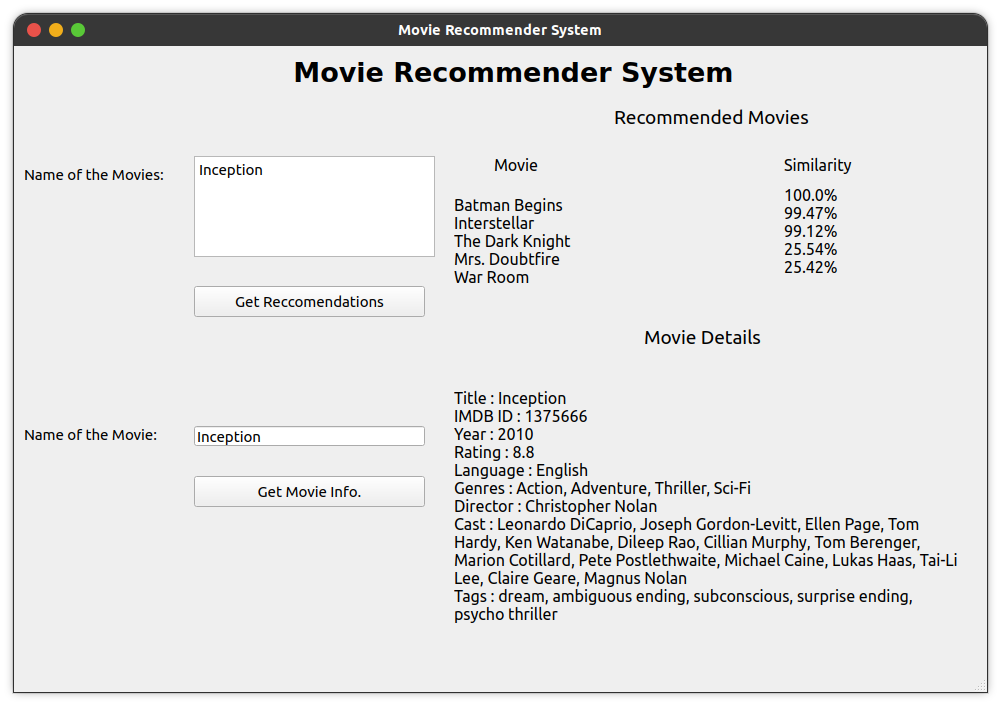
\includegraphics[height=8cm]{gui.png}
\end{figure}
\begin{center}
    \textit{Fig: A screenshot of the recommendation system GUI}
\end{center}
    \hypertarget{introduction}{%
\section{Introduction}\label{introduction}}

Recommender systems are algorithms that attempts to predict user
preferences. For example, recommender systems are used widely by
services such as Spotify and Netflix to recommend songs and movies
respectively to users, based on their past preferences in the respective
domains. Recommender systems have grown significantly, and they are core
parts of various online content providers to the extent that said
content providers offer significant rewards for improvements to their
algorithms. This can be seen in
\href{https://www.kaggle.com/netflix-inc/netflix-prize-data}{Netflix
Prize}.

PageRank is an algorithm used to rank importance of nodes in a network.
It works on the concepts of random walks, wherein a fictional person
traverses the graph at random, and keeps track of the frequency of all
the nodes visited. This eventually converges, and the frequency values
represent relative importance of the nodes in the graph.

\hypertarget{problem}{%
\subsection{Problem}\label{problem}}

The aim for this project was to build a PageRank based movie
recommendation system from first principles. By defining a similarity
parametric for all pairs of movies using publicly available data, and
thus creating an adjacency matrix, we can find the most important movies
in a network using PageRank. Methods of making the recommendation
user-specific are discussed later.

\hypertarget{literature}{%
\subsection{Literature}\label{literature}}

Our main inspiration and source of information were interactive sessions
of CS522 course held during this semester. From there we learnt about
PageRank and various methods of computing it.

\hypertarget{new-idea}{%
\subsection{New Idea}\label{new-idea}}

After learning about PageRank, and it's implementations, we attempted to
use the power iteration method of calculating PageRank to attempt to
build a movie recommendation system.

    \hypertarget{method}{%
\section{Method}\label{method}}

\hypertarget{implementation-details}{%
\subsection{Implementation Details}\label{implementation-details}}

\hypertarget{data-collection-and-processing}{%
\subsubsection{Data Collection and
Processing}\label{data-collection-and-processing}}

The data for this project is all from publicly available sources. Our
first goal was getting a comprehensive set of movies. Initially, we
tried getting \href{https://www.imdb.com/interfaces/}{IMDb data}, but
realised this is only a very small and scattered subset. Eventually, we
found and decided to use the
\href{https://grouplens.org/datasets/movielens/}{GroupLens MovieLens 25M
dataset}, present in the \texttt{ml-25/} directory. This consists of a
relatively small set of around 62k movies, but this was more than enough
for our purposes. In addition to just movies, this dataset also included
for each movie it's title, IMDb ID, year of release, genre(s), tags, and
perhaps most importantly 25 million (hence the name) anonymised user
ratings for the movies. For additional details about the specific data
contained in this dataset, refer to \texttt{ml-25m/README.txt}.

    For additional data about each movie, we built a web scraper that used
the IMDB ID to go to the IMDB URL and extract the relevant information.
Information such as \texttt{Genre}, \texttt{Relevant\ Tags},
\texttt{Director}, \texttt{Cast},\texttt{Language} and \texttt{Rating}
was scraped from the IMDB website for each movie. \texttt{Requests} was
used to get the webpage in HTML format, then \texttt{BeautifulSoup4} was
used to scrape the required data. The script for the scraper can be
found in \texttt{scraped-movies-data/scraper/web\_scraper.py}.

\begin{figure}
    \centering
    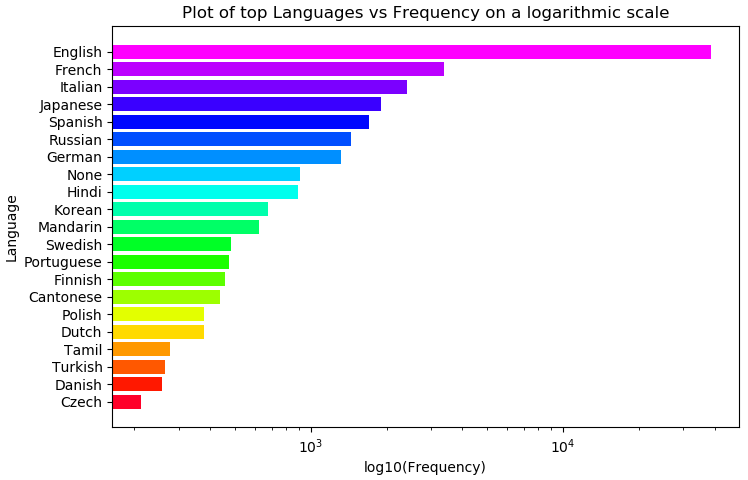
\includegraphics[]{language_count.png}
\end{figure}
\begin{center}
    \textit{Fig: Bar chart displaying frequency of the most common languages in the dataset, on a logarithmic scale}
\end{center}
To clean the movie data and collect it into a proper format,
\texttt{pandas} and \texttt{re} libraries were used to handle the csv
files and process text patterns respectively. This process is present in
\texttt{cleaned\_movies\_generator.py}, and it's output is present in
\texttt{ml-25m/clean\_movies.csv}. Additionally, most of the movies in
the final dataset were irrelvant, primarily because they were of other
languages. Additionally, we could not process the entirety of the data.
For example, a single \(62000\times62000\) matrix of half-precision (2
byte) floats that would represent similarity between movies would take
up over \texttt{7GB} of space. To this end, movies were filtered to
include only those in English, Hindi, Urdu and Punjabi. Additionally,
there were some movies whose IMDb IDs were invalid (the webpage resulted
in a 404 error while scraping) so these movies were dropped. This
resulted in a set of 23843 movies, which are available in
\texttt{processed\_data/cleaned\_subsetted\_movies.csv}.

Additionally, \texttt{ml-25m/ratings.csv} contained in addition to
userID, movieID, and rating, the timestamp for each rating. Since this
was of no use to us, the column was dropped and the resulting dataset is
in \texttt{ml-25m/timeless-ratings.csv}.

    \hypertarget{methodologies-employed}{%
\subsubsection{Methodologies Employed}\label{methodologies-employed}}

\hypertarget{graph-centric}{%
\paragraph{Graph-centric}\label{graph-centric}}

Initially, we tried a graph-centric approach. In this method, the movies
would be nodes on a weighted, undirected graph, and edges would indicate
similar movies, the edge weight being the relative similarity for each
movie. We chose \texttt{graph-tool} as our library of choice since in
comparison to various other libraries, it came out significantly faster
in various
\href{https://www.timlrx.com/2020/05/10/benchmark-of-popular-graph-network-packages-v2/}{Benchmark
tests}.

The plan was to use various parameters of the collected data to create
graphs that represent those similarities. For example, using the user
ratings a graph was created (\texttt{graphs/ratings\_graph.gt.xz}) in
which users and movies were linked by edges weighted with the rating
given to that movie by that user. This was intended to be used to
calculate one similarity parametric between two movies, by using the
fact that similar movies would have fewer edges connecting them, and
these edges would have higher weight. This allowed us to then create a
parametric, where the similarity between two movies (\(S_{u, v}\)) is
directly proportional to the number of shortest paths (\(N_{u, v}\)) (in
terms of number of edges) between two movies, directly proportional to
the average weight along the paths (\(A_{u, v}\)), and inversely
proportional to the number of edges in the paths (\(E_{u, v}\)).
Mathematically, \[S_{u,v} = \frac{N_{u, v}A_{u, v}}{E_{u, v}}\]

\begin{figure}
\centering
    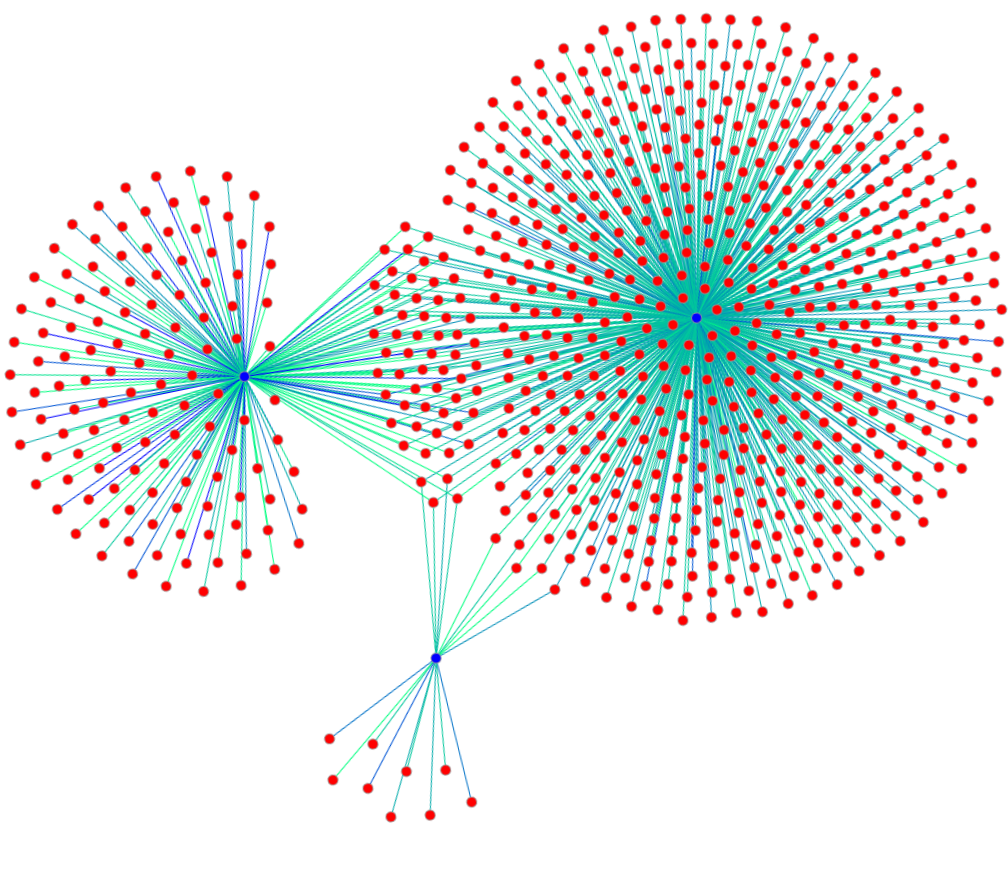
\includegraphics[]{graph.png}
\end{figure}
\begin{center}
    \textit{Fig: Graph of user ratings, where blue nodes at centers are users, red nodes are movies, and edges are weighted by the rating given by user to a movie (shown through colour, green edges indicate higher ratings). This only includes 3 users and the movies they rated.}
\end{center}
This approach quickly fell apart when we constructed the graph, which
turned out to be extremely slow to process, and impossible to run many
centrality or relatedness algorithms on simply due to the large memory
requirements.

\hypertarget{matrix-centric}{%
\paragraph{Matrix-centric}\label{matrix-centric}}

After the lecture on PageRank and calculating it using power iteration,
we attempted to represent movie similarities as matrices. For this, we
identified parameters using which we can compare movies. These are
director, cast, tags, genre, user ratings and language. We attempted to
use \texttt{h5py} library that allows for storing large matrices on disk
as \texttt{.hdf5} files. While this method would have worked in concept,
the processing times were too long since reading from and writing to
disk is a very slow process. It was at this point when we realised that
62000 is too large a set of movies to compute on, even with
low-precision datatypes. As a result, we subsetted the movies as was
described above.

Our goal at this point was to calculate one matrix for each similarity
parameter, and take a linear combination of these matrices to obtain the
final adjacency matrix representing similarities between all pairs of
movies. Director, genre, language and rating similarities were quick to
calculate. In the case of genres, this was due to the fact that there
were very few total genres in the dataset. For director, language, and
rating, the process of computing similarities were not computationally
expensive.

Cast similarity and user similarity had the same issue, that the number
of different users/cast members was too large to compute. Theoretically,
our method would benefit from being able to compute the cast similarity
as well, however due to restriction of our systems this was not
possible. User similarity was incorporated in two different ways.
Firstly, the 20,000 users with the most ratings were used to construct a
user similarity matrix, which was then used to compute an error function
that enabled calculating coefficients of the linear combination through
gradient descent. This method is explained in more detail in the next
section. The second application is used to subset the movies to run
pagerank on. This method is explained in a later section.

All the similarity matrices had different ranges of values, depending on
how they were calculated. Except for director and language similarities,
the matrices also had the issue that larger values represented greater
differences, instead of greater similarities. To rectify this, and
normalize the values, 1 was added to each cell of the matrix, and then
reciprocal of all values was taken. This normalises the values, since 0
cells along the diagonal and other places (indicating 100\% similarity
in that metric) become 1, and larger difference values are less than 1.
This added a constraint on the linear combination coefficients, that
they had to sum to 1 for the scale to remain the same. This is a
workable restriction.

All the similarity matrices can be found in the
\texttt{all\_similarities/} directory. The code to calculate rating
similarity is in
\texttt{all\_similarities/calculation/rating-similarity.py}. For
director similarity, it is in \texttt{director-similarity.py} in the
same directory. The same process was applied for language similarity.
Genre and tags similarity was calculated using the method in
\texttt{similarity-calculator.py}. User similarity was calculated using
\texttt{user-similarity-calculator.py}. Raw, testing code can be found
in \texttt{movie-similarity-generation.ipynb}. The postprocessing code
to add 1 to and calculate reciprocal of the matrices is also present
there.

    \hypertarget{calculation-of-linear-combination-coefficients}{%
\subsubsection{Calculation of Linear Combination
Coefficients}\label{calculation-of-linear-combination-coefficients}}

To calculate the coefficients for the linear combination coefficients of
the similarity matrices, gradient descent was employed. The user
similarity matrix calculated previously was used as a target matrix. The
error function was calculated as the sum of absolute difference between
corresponding values of the adjacency matrix and the user matrix. Using
\texttt{scipy.optimize.minimize} function and
\texttt{method=\textquotesingle{}BFGS\textquotesingle{}} gradient
descent was run from multiple different starting values, and the best
set of weights obtained was used for the final adjacency matrix. The
code for this is available at \texttt{weights-gradient-descent.py}.

    \hypertarget{final-recommendation-system}{%
\subsubsection{Final Recommendation
System}\label{final-recommendation-system}}

After the adjacency matrix was obtained from the coefficients calculated
through gradient descent, PageRank was implemented using the power
iteration method. The input movie names are matched to the ones in our
dataset through fuzzy matching, using \texttt{fuzzywuzzy} library for
Python. This operates by calculating the
\href{https://en.wikipedia.org/wiki/Levenshtein_distance}{Levenshtein
Distance} for each title in our database, given an input title, and
picks the one with the highest value.

After matching movie titles, these are mapped to their respective
\texttt{movieId} values. This is given as input to
\texttt{user\_id.subset()} which subsets around 3000 movies on which the
pagerank algorithm is supposed to be run. To make sure that the
recommendor system is user-specific, the movies are subsetted on the
basis of the movies that are given as input by the user. Genres of the
movies given in the input is used to subset the users. A user-genre
matrix is created, each cell showed the weights (proportional to the
rating they gave to a movie of that genre) of a particular genre as
rated by a particular user. This is then normalized as there are
extremes to the number of movies that a user rated. Final matrix can be
found in \texttt{processed\_data/Scores\_Normalized.csv}. Users who
rated less than 50 movies were removed from this matrix, they were
supposed to be used as test set for gradient descent but later discarded
as this data was not sufficient for calculating the error in similarity
matrix. The users who are top rated for the weighted average of the
genres that is provided as input is returned such that the number of
movies rated by those users is close to 3000. The script for subsetting
the movie can be found in \texttt{user\_id.py}.

A collection is then formed comprising of all the movies rated by all
the given users, along with the input movies. These \texttt{movieId}
values are given to the \texttt{pagerank} function. The function subsets
the adjacency matrix accordingly, makes it Markovian, and performs
PageRank using the power iteration method. To improve locality of
results, a reset probability is introduced. Each column corresponding to
the movies given by the user is given an additional 0.15 weightage, by
the following formula

\[ M' = (1-\alpha)M+\alpha R \] Where \(M'\) is the final matrix on
which PageRank is performed, \(M\) is the raw subsetted matrix, \(R\) is
a matrix of the same dimensions as \(M\) with columns corresponding to
input movies as 1, and \(\alpha=0.15\) is the reset probability

The starting vector for power iteration is taken as
\(v=(1, 0, 0, ..., 0)\), and convergence is achieved when the maximum
difference between corresponding values in successive iterations of
\(v\) is less than tolerance \(\epsilon = 10^{-4}\). Mathematically,
convergence occurs if \[ max(v_i-v_{i-1}) \leq \epsilon \] Where \(v_i\)
is the value of the vector \(v\) after the \(i\)th iteration. A cap of
1000 on iterations was implemented as well, to prevent an infinite loop
in the rare case that convergence does not occur.

The function returns a dictionary mapping \texttt{movieId} to PageRank,
of which the 5 largest values are the recommended movies for the given
input.

    \hypertarget{tools-and-libraries-used}{%
\subsubsection{Tools and Libraries
Used}\label{tools-and-libraries-used}}

All the code for this project is written in Python 3.8.5. The libraries
used in this project and their usages are as follows

(Last column denotes whether library is required to run the recommender
system through \texttt{gui.py})

\begin{longtable}[]{@{}llll@{}}
\toprule
\begin{minipage}[b]{0.22\columnwidth}\raggedright
Library\strut
\end{minipage} & \begin{minipage}[b]{0.22\columnwidth}\raggedright
Usage\strut
\end{minipage} & \begin{minipage}[b]{0.22\columnwidth}\raggedright
Link\strut
\end{minipage} & \begin{minipage}[b]{0.22\columnwidth}\raggedright
Required\strut
\end{minipage}\tabularnewline
\midrule
\endhead
\begin{minipage}[t]{0.22\columnwidth}\raggedright
\texttt{numpy==1.19.4}\strut
\end{minipage} & \begin{minipage}[t]{0.22\columnwidth}\raggedright
Various mathematical applications, including handling of very large
matrices, matrix multiplication, and various other matrix
operations\strut
\end{minipage} & \begin{minipage}[t]{0.22\columnwidth}\raggedright
\url{https://numpy.org/}\strut
\end{minipage} & \begin{minipage}[t]{0.22\columnwidth}\raggedright
Yes\strut
\end{minipage}\tabularnewline
\begin{minipage}[t]{0.22\columnwidth}\raggedright
\texttt{matplotlib==3.1.2}\strut
\end{minipage} & \begin{minipage}[t]{0.22\columnwidth}\raggedright
For data visualizations\strut
\end{minipage} & \begin{minipage}[t]{0.22\columnwidth}\raggedright
\url{https://matplotlib.org/}\strut
\end{minipage} & \begin{minipage}[t]{0.22\columnwidth}\raggedright
No\strut
\end{minipage}\tabularnewline
\begin{minipage}[t]{0.22\columnwidth}\raggedright
\texttt{scipy==1.3.3}\strut
\end{minipage} & \begin{minipage}[t]{0.22\columnwidth}\raggedright
Used \texttt{scipy.optimize} to perform gradient descent and find
optimal combination of weights for different similarity parameters\strut
\end{minipage} & \begin{minipage}[t]{0.22\columnwidth}\raggedright
\url{https://www.scipy.org/}\strut
\end{minipage} & \begin{minipage}[t]{0.22\columnwidth}\raggedright
No\strut
\end{minipage}\tabularnewline
\begin{minipage}[t]{0.22\columnwidth}\raggedright
\texttt{pandas==1.1.3}\strut
\end{minipage} & \begin{minipage}[t]{0.22\columnwidth}\raggedright
For handling and processing of raw and processed data, in the form of
\texttt{.csv} files\strut
\end{minipage} & \begin{minipage}[t]{0.22\columnwidth}\raggedright
\url{https://pandas.pydata.org/}\strut
\end{minipage} & \begin{minipage}[t]{0.22\columnwidth}\raggedright
Yes\strut
\end{minipage}\tabularnewline
\begin{minipage}[t]{0.22\columnwidth}\raggedright
\texttt{re}\strut
\end{minipage} & \begin{minipage}[t]{0.22\columnwidth}\raggedright
Python Regular Expressions library for pattern matching while processing
raw data\strut
\end{minipage} & \begin{minipage}[t]{0.22\columnwidth}\raggedright
\url{https://docs.python.org/3/library/re.html}\strut
\end{minipage} & \begin{minipage}[t]{0.22\columnwidth}\raggedright
No\strut
\end{minipage}\tabularnewline
\begin{minipage}[t]{0.22\columnwidth}\raggedright
\texttt{numba==0.51.2}\strut
\end{minipage} & \begin{minipage}[t]{0.22\columnwidth}\raggedright
A Python compiler that allows for compiling a subset of python and numpy
to machine code, used while testing methods and processing data to
accelerate some computations\strut
\end{minipage} & \begin{minipage}[t]{0.22\columnwidth}\raggedright
\url{https://numba.pydata.org/}\strut
\end{minipage} & \begin{minipage}[t]{0.22\columnwidth}\raggedright
No\strut
\end{minipage}\tabularnewline
\begin{minipage}[t]{0.22\columnwidth}\raggedright
\texttt{graph-tool}\strut
\end{minipage} & \begin{minipage}[t]{0.22\columnwidth}\raggedright
A Python library written in C++ for handling graphs, used while testing
different methods of PageRank and methods of processing movie
similarity. This was eventually not used in the final result, and is not
required to run the recommender system\strut
\end{minipage} & \begin{minipage}[t]{0.22\columnwidth}\raggedright
\url{https://graph-tool.skewed.de/}\strut
\end{minipage} & \begin{minipage}[t]{0.22\columnwidth}\raggedright
No\strut
\end{minipage}\tabularnewline
\begin{minipage}[t]{0.22\columnwidth}\raggedright
\texttt{lxml}\strut
\end{minipage} & \begin{minipage}[t]{0.22\columnwidth}\raggedright
A Python library that aids in processing large XML and HTML files\strut
\end{minipage} & \begin{minipage}[t]{0.22\columnwidth}\raggedright
\url{https://lxml.de/}\strut
\end{minipage} & \begin{minipage}[t]{0.22\columnwidth}\raggedright
No\strut
\end{minipage}\tabularnewline
\begin{minipage}[t]{0.22\columnwidth}\raggedright
\texttt{BeautifulSoup==4.9.0}\strut
\end{minipage} & \begin{minipage}[t]{0.22\columnwidth}\raggedright
Beautiful Soup is a library that helps to scrape information from web
pages, used while scraping the IMDB site for data.\strut
\end{minipage} & \begin{minipage}[t]{0.22\columnwidth}\raggedright
\url{https://pypi.org/project/beautifulsoup4/}\strut
\end{minipage} & \begin{minipage}[t]{0.22\columnwidth}\raggedright
No\strut
\end{minipage}\tabularnewline
\begin{minipage}[t]{0.22\columnwidth}\raggedright
\texttt{fuzzywuzzy==0.18.0}\strut
\end{minipage} & \begin{minipage}[t]{0.22\columnwidth}\raggedright
Used for fuzzy matching of input movie names to those in our
dataset\strut
\end{minipage} & \begin{minipage}[t]{0.22\columnwidth}\raggedright
\url{https://pypi.org/project/fuzzywuzzy/}\strut
\end{minipage} & \begin{minipage}[t]{0.22\columnwidth}\raggedright
Yes\strut
\end{minipage}\tabularnewline
\begin{minipage}[t]{0.22\columnwidth}\raggedright
\texttt{python-Levenshtein}\strut
\end{minipage} & \begin{minipage}[t]{0.22\columnwidth}\raggedright
Used by \texttt{fuzzywuzzy} to accelerate calculation of Levenshtein
distance\strut
\end{minipage} & \begin{minipage}[t]{0.22\columnwidth}\raggedright
\url{https://github.com/ztane/python-Levenshtein/}\strut
\end{minipage} & \begin{minipage}[t]{0.22\columnwidth}\raggedright
Yes\strut
\end{minipage}\tabularnewline
\begin{minipage}[t]{0.22\columnwidth}\raggedright
\texttt{PyQt5}\strut
\end{minipage} & \begin{minipage}[t]{0.22\columnwidth}\raggedright
PyQt is a Python binding of the cross-platform GUI toolkit Qt,
implemented as a Python plug-in, used for making a GUI to run the
programme\strut
\end{minipage} & \begin{minipage}[t]{0.22\columnwidth}\raggedright
\url{https://pypi.org/project/PyQt5/}\strut
\end{minipage} & \begin{minipage}[t]{0.22\columnwidth}\raggedright
Yes\strut
\end{minipage}\tabularnewline
\bottomrule
\end{longtable}

    \hypertarget{results}{%
\section{Results}\label{results}}

\hypertarget{experiment-findings}{%
\subsection{Experiment Findings}\label{experiment-findings}}

The final adjacency matrix obtained is \texttt{final\_adj\_mat.npz}. The
weights used to obtain this were \((0.873, 0.047, 0.08)\) for director,
genre, and tags similarity respectively. Including additional matrices
took a long time to compute, and for the time we were able to run, the
error was higher. Additionally. It was found that Drama and Comedy
movies seem to dominate the recommendations. The recommendation system
can be interacted through the GUI app, by running \texttt{gui.py}.

\hypertarget{interpretation-of-findings}{%
\subsection{Interpretation of
Findings}\label{interpretation-of-findings}}

Observing the weight values, it appears as though director similarity is
given a surprisingly high weightage. This may make some sense, since
directors often make similar types of movies. Genres was also
surprisingly given a fairly low weightage. This could possibly be
because tags serve a similar purpose, and since there are a larger
number of tags, the granularity of similarity values would be much more,
and consequently less polarising.

Upon exploration, it appeared that Drama and Comedy were very frequent
genres in our dataset. Due to this, while using \texttt{user-id.subset}
they have disproportionately higher influence on the subsetted users.
This tends to bias the recommendations towards movies with these genres,
since they are the ones subsetted. Currently, movies without these tags
have better recommendations.

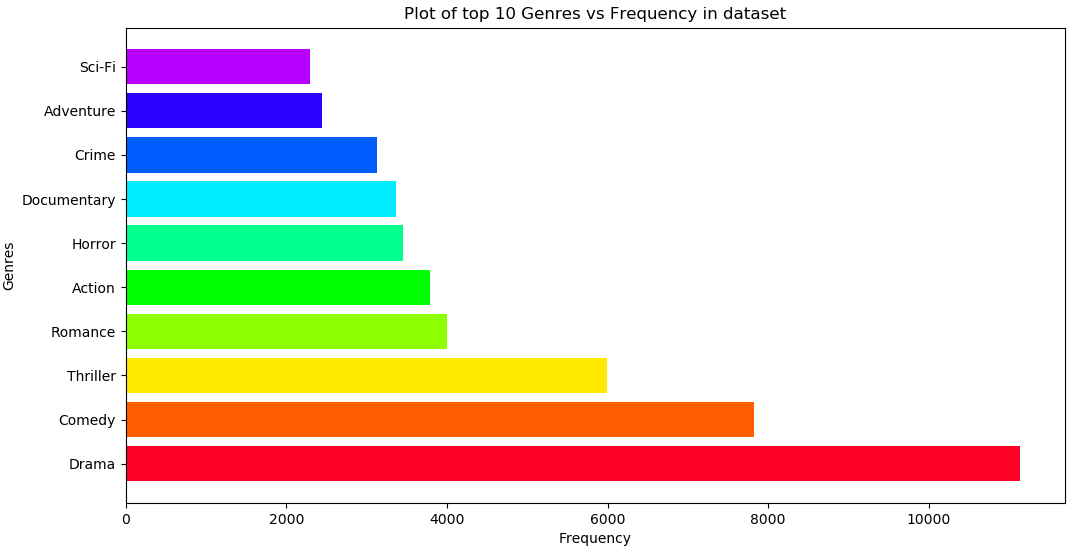
\includegraphics[]{genre_count.png}
\begin{center}
    \textit{Fig: Bar chart displaying frequency of the top 10 genres in the dataset we used, on a linear scale. Visibly, Comedy and Drama genres are exceptionally frequent}
\end{center}
    \hypertarget{conclusion}{%
\section{Conclusion}\label{conclusion}}

PageRank appears to be a workable technique for building a
recommendation system. It may be possible to improve the system further
if larger data can be processed, but this project can serve as a proof
of concept for such an approach. There are definitely various
improvements that can be made to the approaches we have taken to process
and use our data, but the current approach has also provided us with
workable results. Some improvements could be in the form of finding an
appropriate normalization for different frequencies of genres, to avoid
biasing. Additionally, the algorithm could be significantly improved if
additional data and the other matrices are able to be processed and used
in the similarity metric. We did not have a deep understanding of the
various methods of gradient descent, and perhaps a better method,
implemented appropriately, could have offered better results. In
relation to this, there could be significant improvements to the error
function used for gradient descent.

This project was a major learning experience, in various aspects of data
analysis and recommendation systems. We learnt to scrape web data,
process data with pandas and numpy, storing and manipulating large data,
build GUIs, and applications of scientific techniques like gradient
descent.

\hypertarget{team-work}{%
\subsection{Team Work}\label{team-work}}

This project was definitely a huge group effort. We managed to
effectively split the workload by distributing different tasks, and
combining the results. Another method of collaboration was splitting the
computation. For time consuming processes, like scraping web data, we
were able to effectively halve the total time by each doing half the
computation. This was applied not only for scraping web data, but also
calculating tags and user similarity matrices, and running gradient
descent for various input weights to find the best combination of
coefficients.

Not only just computation and effort, but ideas are also much better
with groups. We were able to effectively find faults in each other's
ideas, to identify areas of improvement, and effective methods of
building a better recommendation system. The project involved not only a
lot of coding, but a lot of discussions held online to find solutions to
various problems encountered. We also spent large amounts of time
exploring and getting to understand the data, then sharing our findings
to think of better pipelines to process our data.


    % Add a bibliography block to the postdoc
    
    
    
\end{document}
